%!TeX root=../tese.tex
%("dica" para o editor de texto: este arquivo é parte de um documento maior)
% para saber mais: https://tex.stackexchange.com/q/78101/183146

\chapter{Dynamic Analysis}
\label{cap:dynamic}

Following the static analysis, it became clear that a dynamic analysis would be
of the utmost importance. Understanding how the recommendation model responds to
users reinforcing its internal biases, like the ones already detected, could
potentially lead to a better understanding of how these systems favor certain
kinds of content.

In order for this analysis to be more true to reality, we implemented a simple
recommendation algorithm using TensorFlow Recommenders \citep{}, a library for
machine learning developed by Google for use with its TensorFlow \citep{}
framework. This means that, even though our model is deliberately bare-bones, it
conforms to industry-standard technology and practices.

The choice to use a simple recommendation algorithm instead of a more complex
one was twofold: first, we didn't want to use a model that could introduce many
confounding parameters to the analysis (e.g. hyperparameters, hardware
requirements, etc.), and second, we wanted to study a baseline that could, in
the future, be used as a comparison point for more complex algorithms.

The goal of this analysis is to gather data on how the recommendation system
behaves over time. As will be explained in the next sections, is to understand
what happens to the recommendation profile of the algorithm as it interacts with
itself via users that follow the generated suggestions.

The expectation is that the recommendation profile will grow ever more steep,
which is a reasonable guess; if the users reinforce the beliefs of the
algorithm, then is stands to reason that it will recommend popular movies with
more and more frequently, to more and more users. How much more frequently,
however, is the true question.

For the sake of clarity, let's imagine two users with very distinct preferences:
Alice, who enjoys adventure movies, and Bob, who enjoys horror movies. In
principle, the algorithm should have very different recommendations for both of
them and, were they to follow them, their custom suggestions should grow
increasingly different. At the end of this experiment, users like Alice would
all be recommended the same movies, and users like Bob would have their own set
of very popular films; we should expect, therefore, a multimodal distribution of
the recommendation frequencies, with "typical" adventure movies and "typical"
horror movies being much more popular than comedy, for example.

However, if the final recommendation profile looked like what was showcased in
the previous chapter, i.e. a very small subset of movies being recommended to
most users, then we could infer that the system devolved into a degenerate
feedback loop, ignoring personal preferences and distinctions between films.

\section{Datasets}
\label{sec:datasets04}

For the dynamic experiments, we kept using the Movielens dataset \citep{}. This
time, however, we used the full ``1M'' dataset instead of sampling movies from
the larger ``25M'' version. Given that we wanted our dynamic analysis to be
conducted in a realistic scenario, we decided that it would be better not to
change the data. This whole experiment will, therefore, use a version of the
dataset commonly used for machine learning benchmarks with no alteration
whatsoever.

The 1M dataset contains 1,000,209 ratings of almost 4000 movies made by over
6000 anonymous MovieLens users who joined the platform in 2000. In this
particular version, each user has made at least 20 ratings. There are 4 columns
available:

\begin{itemize}
  \item \verb|UserID|: Unique user identifier, ranging from 1 to 6040.
  \item \verb|MovieID|: Unique movie identifier, ranging from 1 to 3952.
  \item \verb|Rating|: Movie rating according to user, from 0 to 5 stars.
  \item \verb|Timestamp|: When the user made the rating, in seconds since the
  epoch.
\end{itemize}

A second, auxiliary, dataset was also used to enrich the main one. ``Movies''
contains extra information about the movies in 1M, which allowed us to add more
variables to the recommendation system. This new dataset has 3 columns:

\begin{itemize}
  \item \verb|MovieID|: Unique user identifier, ranging from 1 to 6040.
  \item \verb|Title|: Title of the movie, as provided by IMDB.
  \item \verb|Genres|: Pipe-separated string with all applicable genres.
\end{itemize}

The other accompanying dataset, ``Users'', has not been used for the purposes of
this analysis. The reasoning behind this decision will be explained in greater
detail in the next section.

\section{Experiments}
\label{sec:experiments04}

% Explicar aqui no começo o que é um modelo estatístico, talvez fazer um capítulo

The dynamic experiment starts in a manner much similar to the static experiment.
The full MovieLens dataset is fed as training data to a recommendation system in
order to get it ready for giving suggestions to users. As explained in the
opening section of this chapter, we chose a simple algorithm in order to reduce
the number of possible interferences architecture could have on our analysis.

The chosen recommendation algorithm was a basic ranking model described in
\citet{} using TensorFlow Recommenders \citep{}. It is composed of multiple
stacked dense layers and uses mean squared error as its loss function. The main
class in the model is reproduced below, and the full algorithm is listed in
Appendix~\ref{}.

%% Deixar o código em pseudo-código para ficar mais claro

\begin{verbatim}
class MovielensModel(tfrs.models.Model):

  def __init__(self):
    super().__init__()
    self.ranking_model: tf.keras.Model = RankingModel()
    self.task: tf.keras.layers.Layer = tfrs.tasks.Ranking(
      loss = tf.keras.losses.MeanSquaredError(),
      metrics=[tf.keras.metrics.RootMeanSquaredError()]
    )

  def call(self, features: Dict[str, tf.Tensor]) -> tf.Tensor:
    return self.ranking_model(
        (features["user_id"], features["movie_title"]))

  def compute_loss(self, features: Dict[Text, tf.Tensor],
                    training=False) -> tf.Tensor:
    labels = features.pop("user_rating")

    rating_predictions = self(features)

    # The task computes the loss and the metrics.
    return self.task(labels=labels, predictions=rating_predictions)
\end{verbatim}

In the first step of the experiment, we trained the recommendation model using
Movielens' 1M ratings dataset, which we will refer to as \verb|ratings0| from
now on. All available data was used and, in the end, we achieved a root mean
squared error (RMSE) of 0.92; this result is similar to TFRS' deep \& cross
network \citep{} results when trained on the same data. Once \verb|model0| was
ready for making recommendations, we applied it to every possible user-movie
pairing, generating a complete matrix of predicted ratings called
\verb|predictions0|.

In an environment like YouTube's recommendations sidebar, the user is presented
with a few items that the algorithm thinks they would like, and then they can
either ignore the sidebar or select one of the options to watch. Since our goal
was to explore what would happen when the recommendation system entered a
feedback loop, we picked one movie at random from each user's 10 best-ranked
entries.

This set of well-ranked movies was our way of simulating thousands of users
simultaneously approving of the algorithms recommendations and selecting one
option from their sidebars. The last step involved removing the oldest rating of
each each user from \verb|ratings0| and appending these these selections to the
dataset in order to create \verb|ratings1|. The full data flow is illustrated
in Figure~\ref{fig:fig04_dynamic_diagram}

\begin{figure}
  \centering
  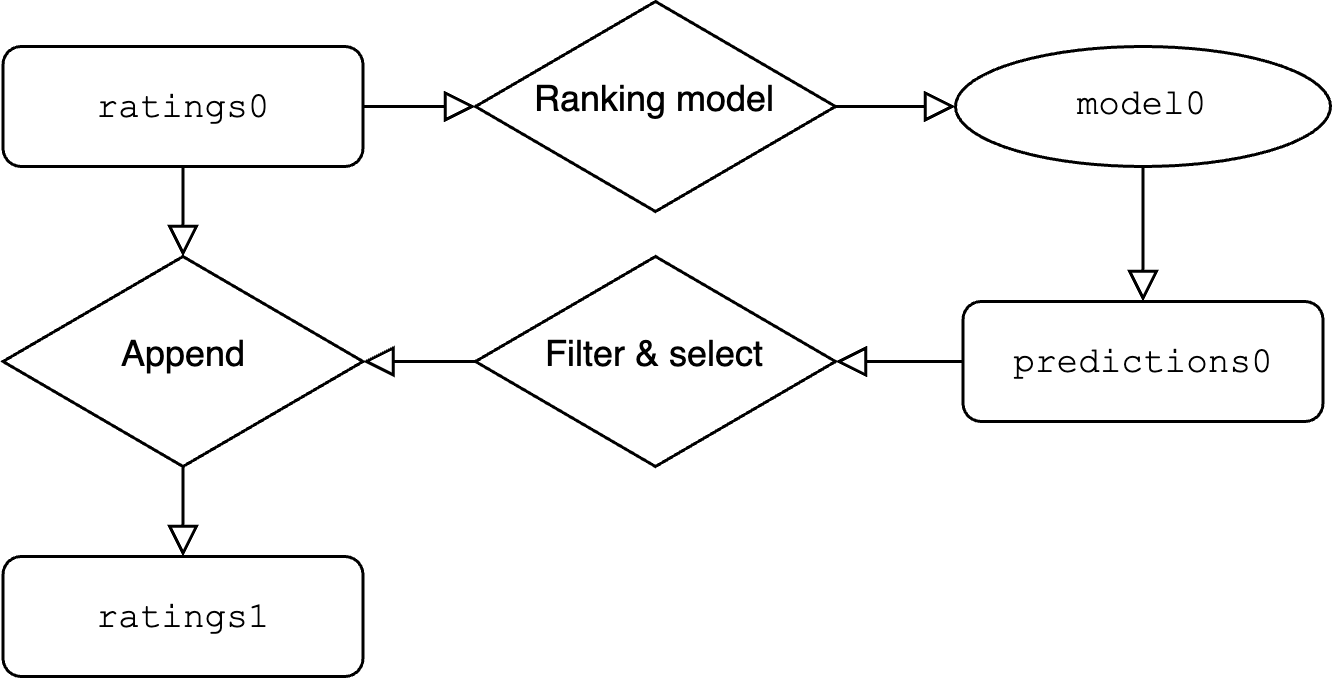
\includegraphics[width=\textwidth]{04_dynamic_diagram}
  \caption{Data flow diagram.\label{fig:fig04_dynamic_diagram}}
\end{figure}

% Explicar o que são os formatos no caption da figura.

A feedback loop, however, can't be created from a single iteration. For this
reason, the process just described was classified as the ``zeroth'' iteration in
the process (as it involved \verb|ratings0|). The ``first'' iteration began with
\verb|ratings1|, trained \verb|model1|, generated \verb|predictions1|, and ended
with \verb|ratings2|. We repeated this process until we got to \verb|ratings4|,
totaling 5 ratings datasets (one original and 4 derived through ranking models).

A simplified version of the R code that created \verb|ratingsN+1| from
\verb|ratingsN| can be found below. The omitted functions served mostly
auxiliary purposes which made the datasets conform to TensorFlow's format
expectations. The full code is listed in Appendix~\ref{}.

\begin{verbatim}
predictions |>
  group_by(user_id) |>
  slice_max(prediction, n = 10) |>
  slice_sample(n = 1) |>
  ungroup() |>
  bind_rows(old_ratings) |>
  group_by(user_id) |>
  slice_max(timestamp, n = -1, with_ties = FALSE) |>
  ungroup()
\end{verbatim}

With these new datasets we were able to analyze the differences between distinct
generations of models and understand exactly how the positive feedback loop
influenced the last iteration.

A series of analysis were conducted using these datasets as sources. We found
that, with each iteration, the recommendation profile got steeper and steeper,
that is, a few popular items got more recommended while the rest fell into
disfavor; this was predictably more noticeable in movies with higher average
ratings. In fact, a small set of around 20 movies were the only ones that
consistently rose in popularity with new iterations.

Figure~\ref{fig:fig04_profile_grouped} has five subplots which represent each
iteration of the recommendation system. For \verb|ratings0|, it's possible to
see that a number of well-rated movies were more popular, i.e., were rated by
more people. Once we generate the first batch of recommendations, we add up the
number of users each movie was recommended to; this is seen in the second plot,
\verb|ratings1|. We can clearly see that a small subset of movies strayed from
the pack and to more people that had watched them previously.

This process repeats itself until, in \verb|ratings4|, the most popular movie is
recommended more than 2000 times, while the most popular movie in
\verb|ratings0| was watched a little over 500 times.

As explained before, we expected that movies which where already popular would
be recommended more times, but these plots indicate a powerful feedback loop.
Examining the data, we saw that the algorithm was consistently recommending
movies which the users had already watched and this process only became more
accentuated with each subsequent iteration.

\begin{figure}
  \centering
  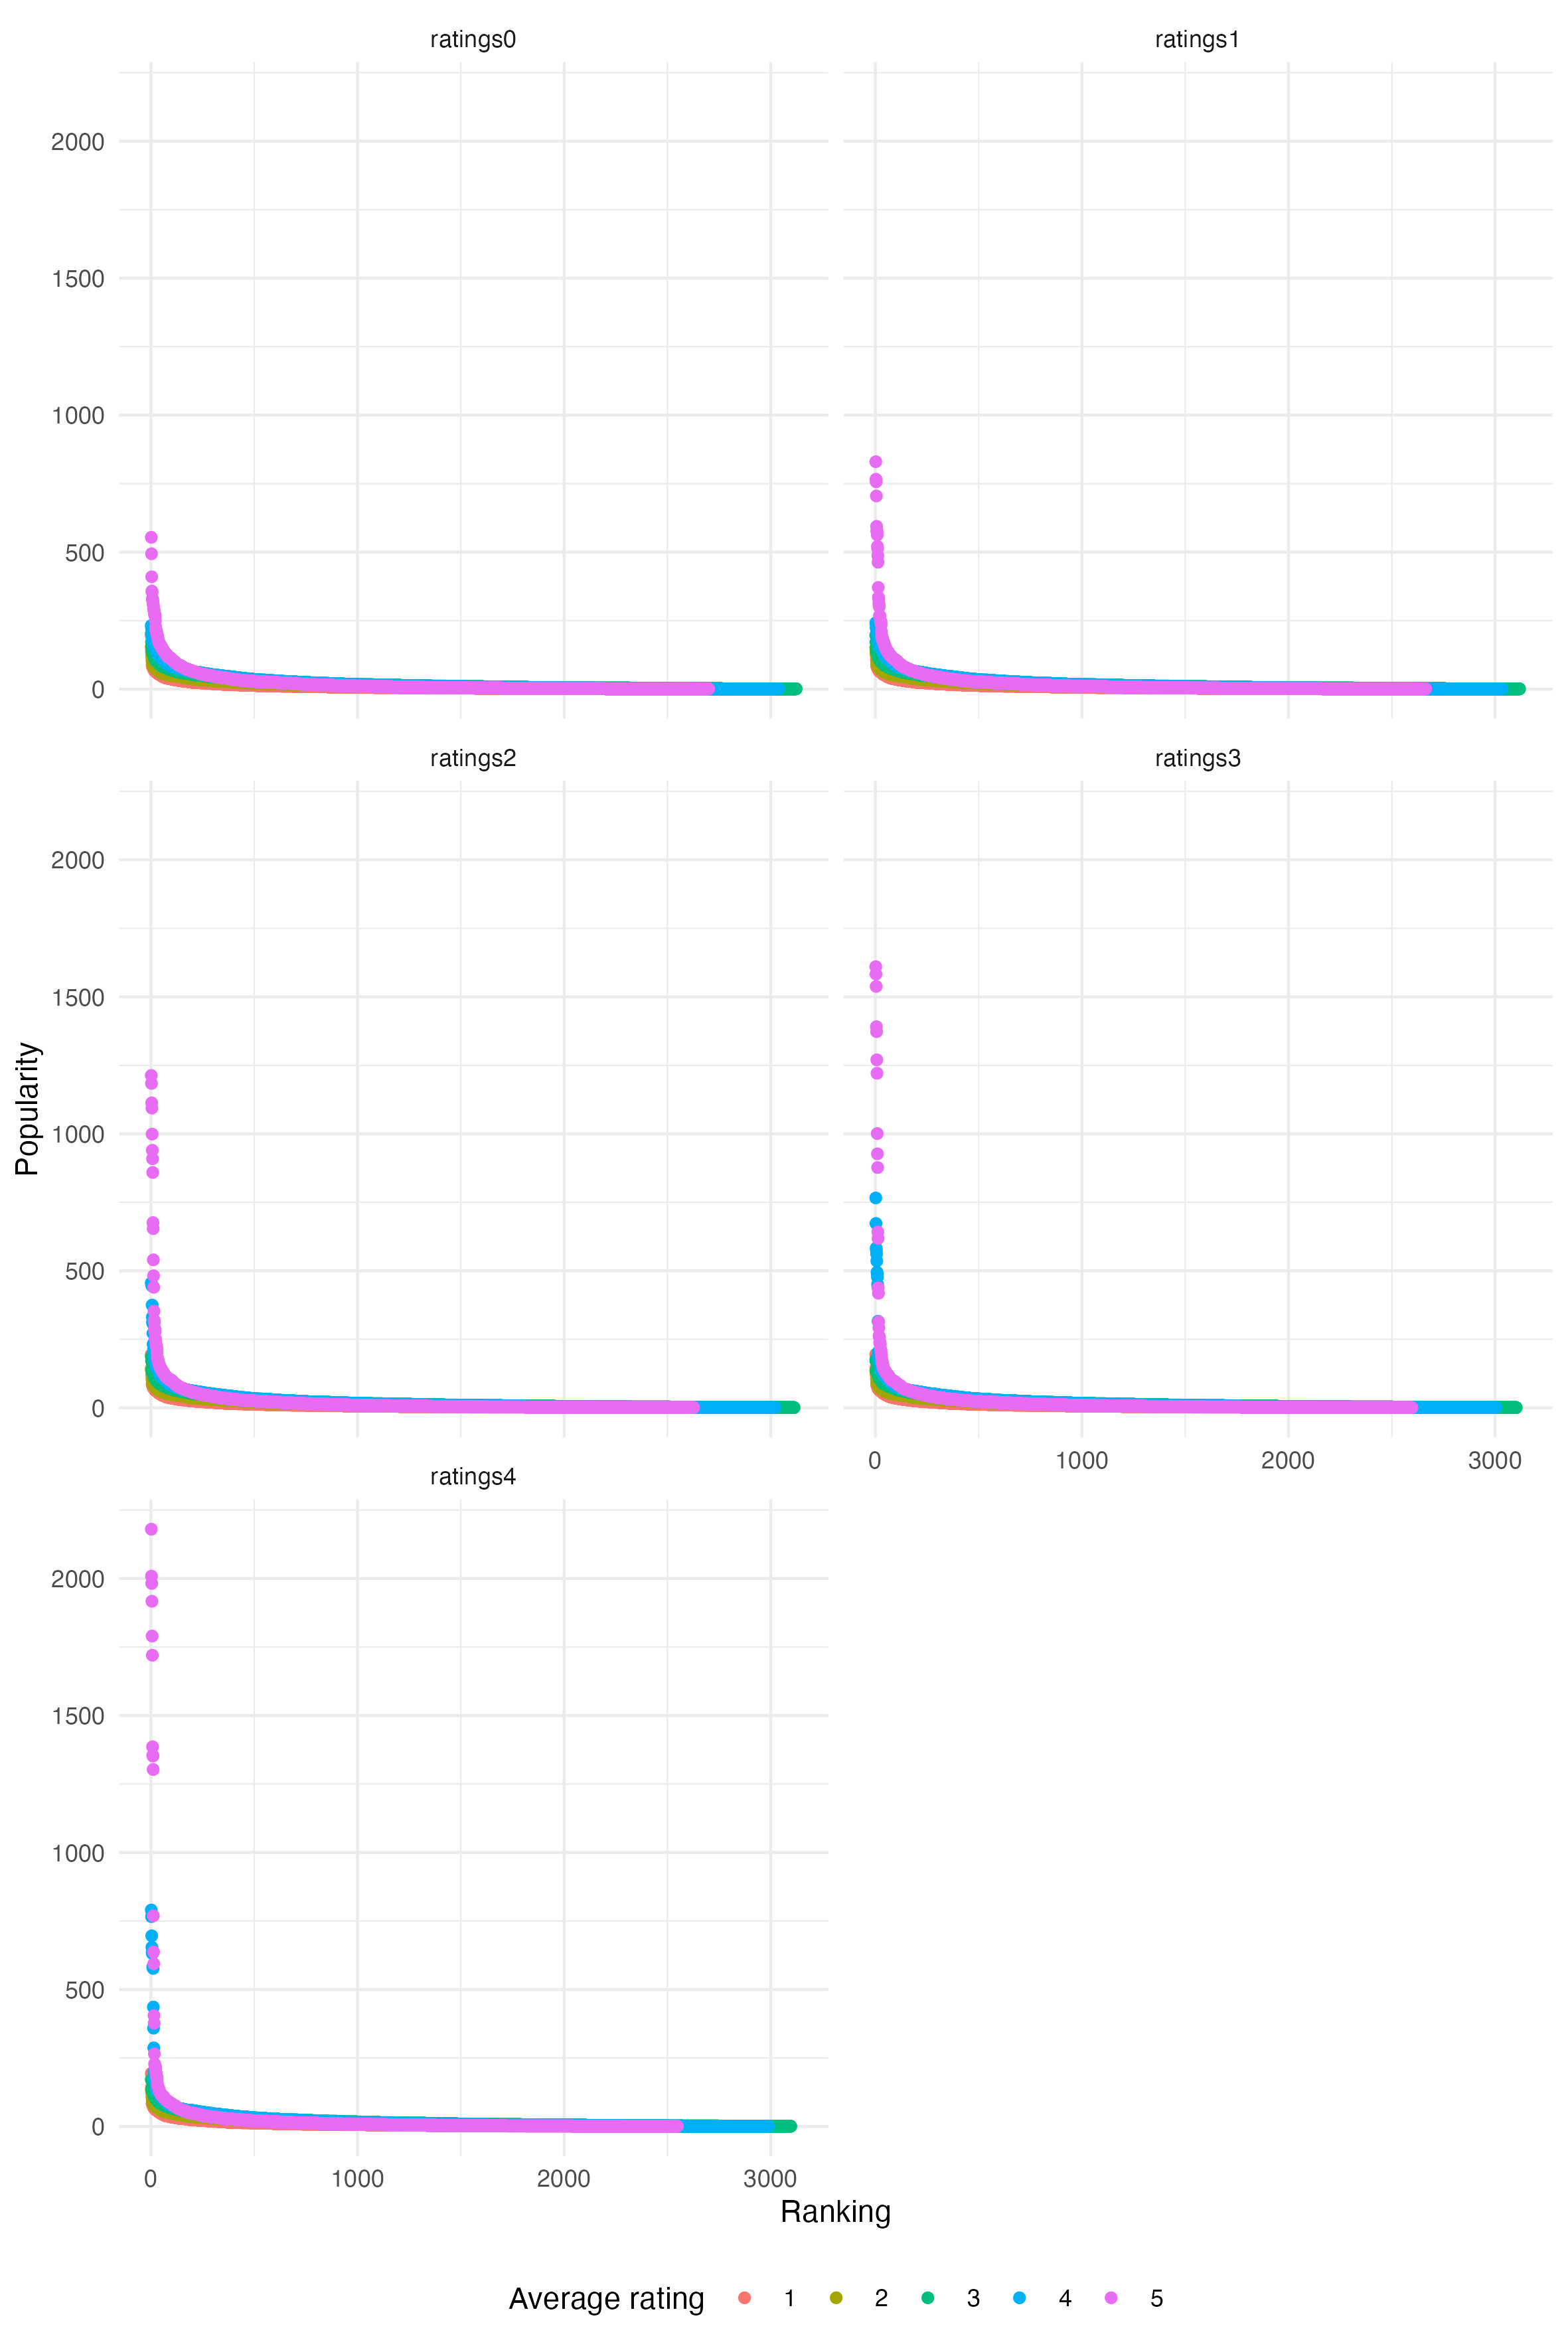
\includegraphics[width=\textwidth]{04_profile_grouped}
  \caption{Recommendation profile of every generation. Colors indicate average
  movie rating, which is a strong predictor of popularity over time.
  \label{fig:fig04_profile_grouped}}
\end{figure}

A good way to measure how diverse were the recommendations made by the algorithm
is to calculate the entropy \citep{} of each set. In the extreme, if the same
movie is recommended to every user, than the entropy of the recommendations will
tend to zero. In absolute terms, the entropy of \verb|ratings0| was 7.42, and
the entropy of \verb|ratings4| was 6.08 (82\% lower). A comparison in relative
terms is displayed in Figure~\ref{fig:fig04_entropy}.

\begin{figure}
  \centering
  \begin{subfigure}{0.45\textwidth}
    \centering
    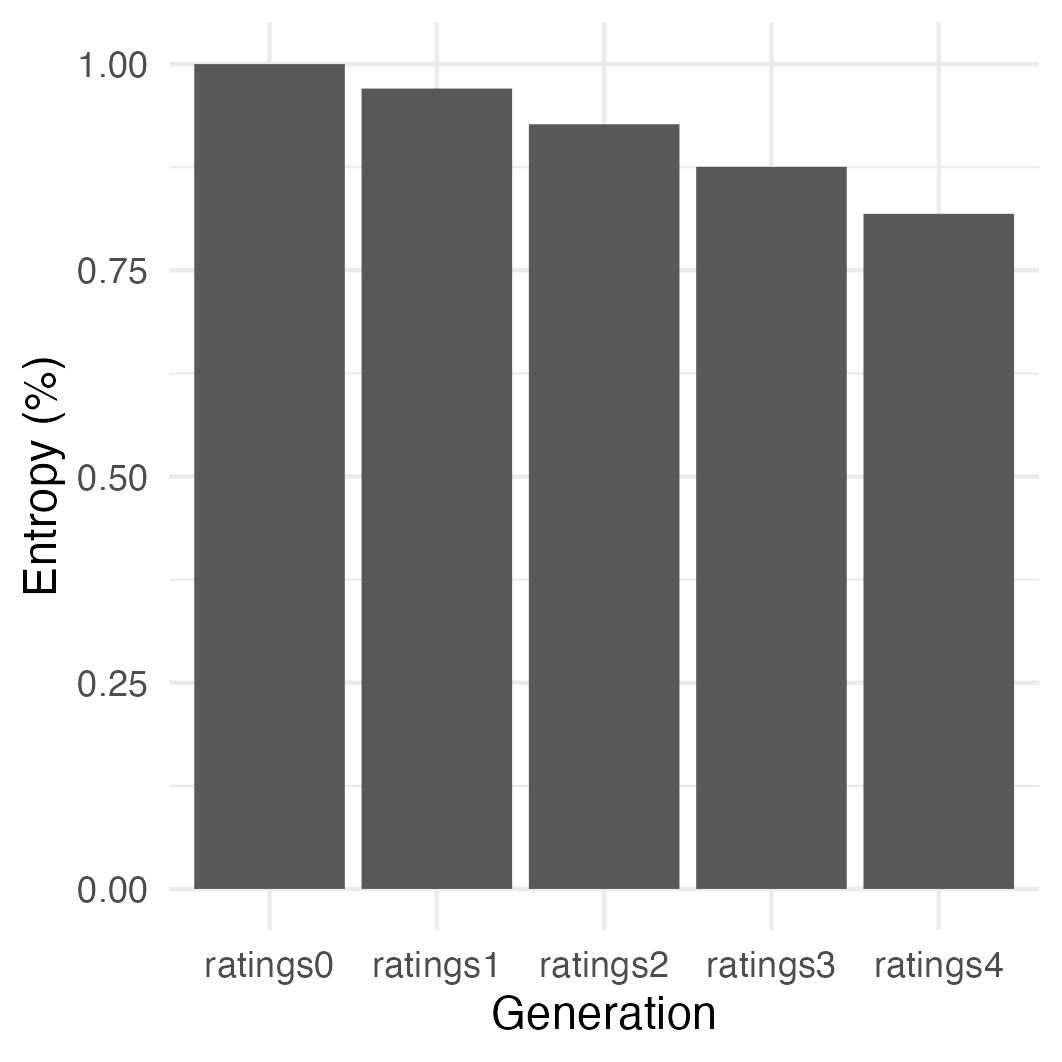
\includegraphics[width=\textwidth]{04_entropy}
  \end{subfigure}
  \caption{Recommendation entropy as a percentage of ratings0s entropy.
  \label{fig:fig04_entropy}}
\end{figure}

We can also observe this reduction of variety in an even more visual way. In
Figure~\ref{fig:fig04_popularity_time_both} we plotted movie popularity over
time; each line represents a movie and each step in the x-axis is a new
generation of the model. Figure~\ref{fig:fig04_popularity_time} makes it very
clear that no more than 15 movies rose in popularity over the four generations
of the recommendation system, becoming orders of magnitude more popular than the
rest. We also scaled the y-axis by taking the its log in
Figure~\ref{fig:fig04_log_popularity_time}, and we can see that, in fact, no
other movie rose in popularity besides the ones that stick out after
\verb|model2|.

It is also of note that the few movies that rise in popularity are not the most
popular ones from \verb|ratings0|, even though genre was the only metadata we
fed into the system. This uncovers a significant feature of the feedback loop we
observed in Figure~\ref{fig:fig04_profile_grouped}: the items that the algorithm
amplifies don't necessarily have to be the most mainstream, or in other words,
recommendation systems are able to boost content artificially.

\begin{figure}
  \centering
  \begin{subfigure}{0.45\textwidth}
    \centering
    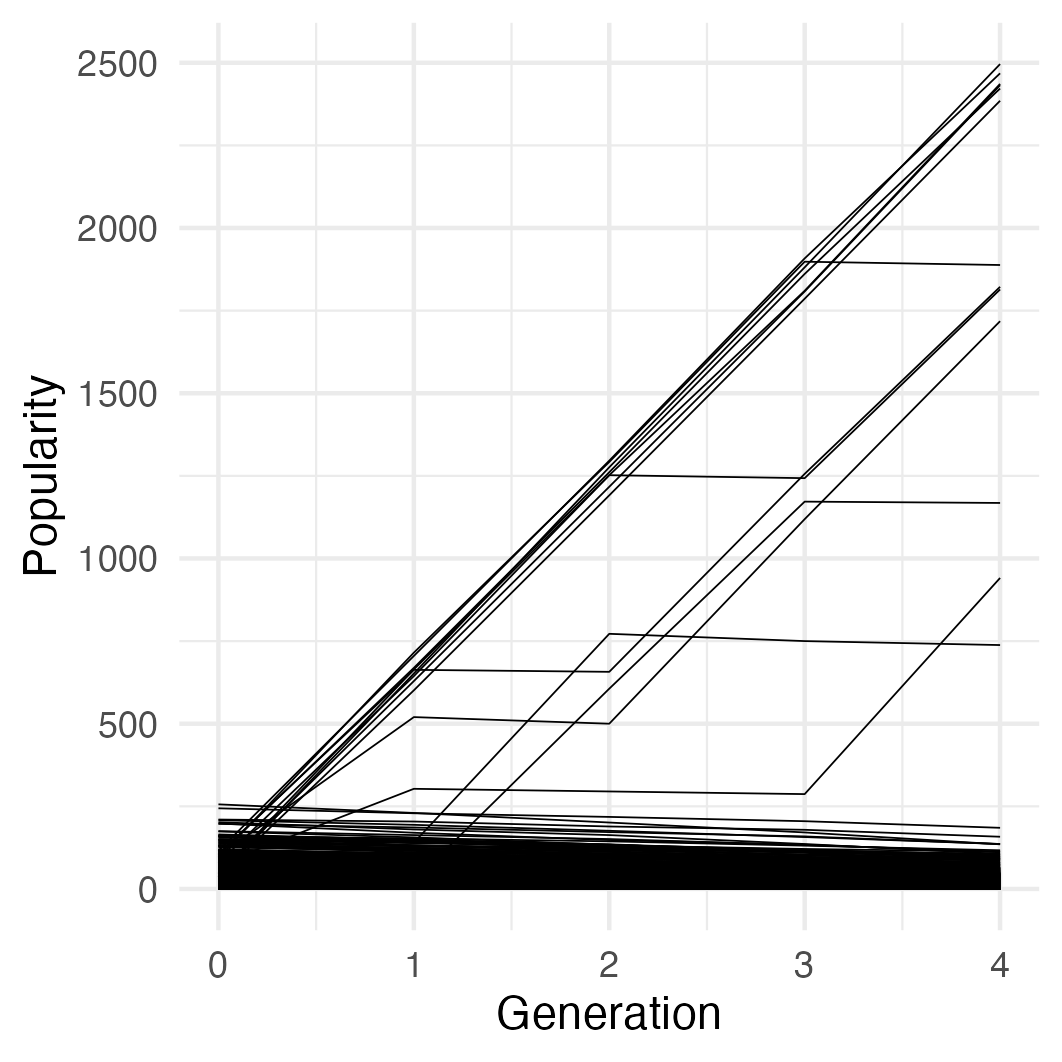
\includegraphics[width=\textwidth]{04_popularity_time}
    \caption{Movie popularity over time.\label{fig:fig04_popularity_time}}
  \end{subfigure}
  \begin{subfigure}{0.45\textwidth}
    \centering
    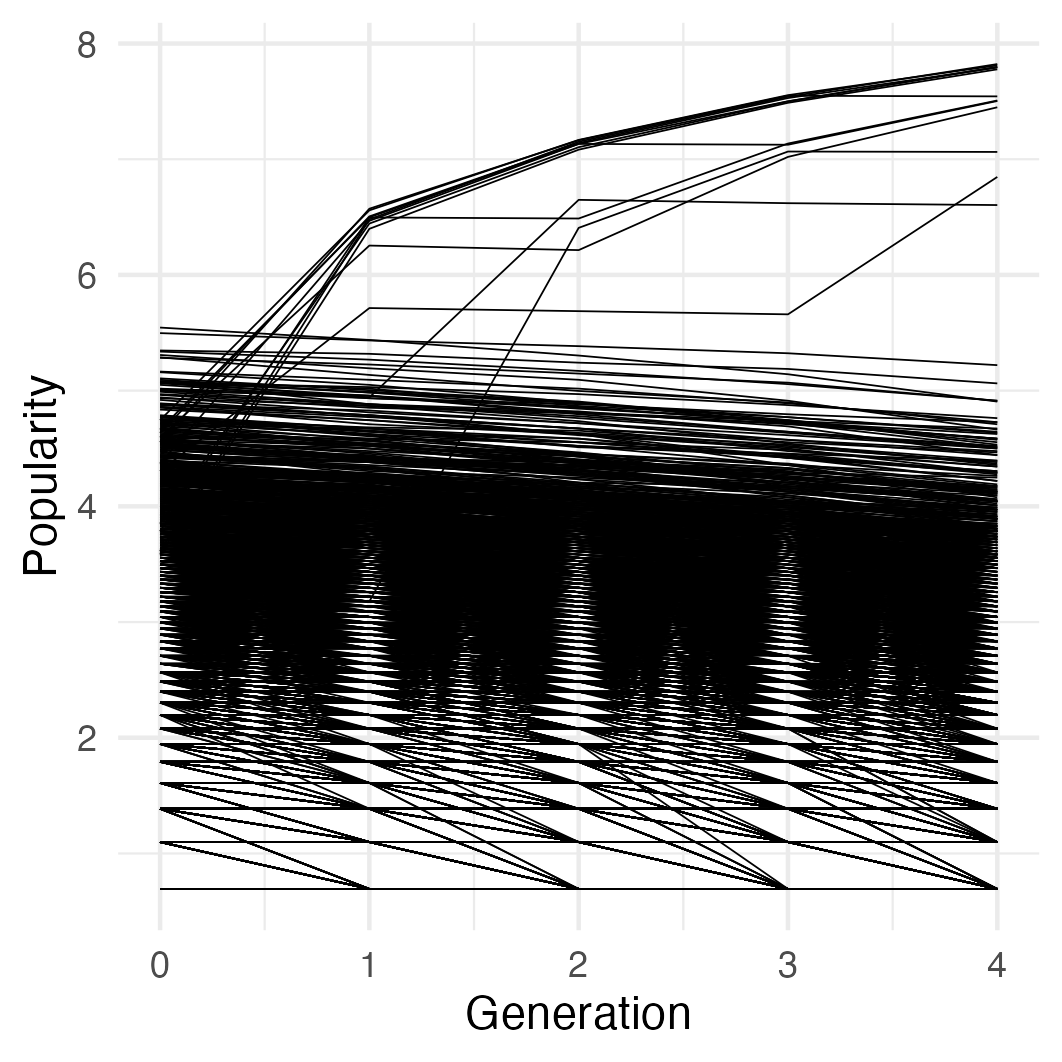
\includegraphics[width=\textwidth]{04_log_popularity_time}
    \caption{Movie log-popularity over time.\label{fig:fig04_log_popularity_time}}
  \end{subfigure}
  \caption{Popularity of every movie from ratings0 to ratings4.\label{fig:fig04_popularity_time_both}}
\end{figure}

% explicar que, nos gráficos, popularidade significa número de recs para t = 1..4

\begin{figure}
  \centering
  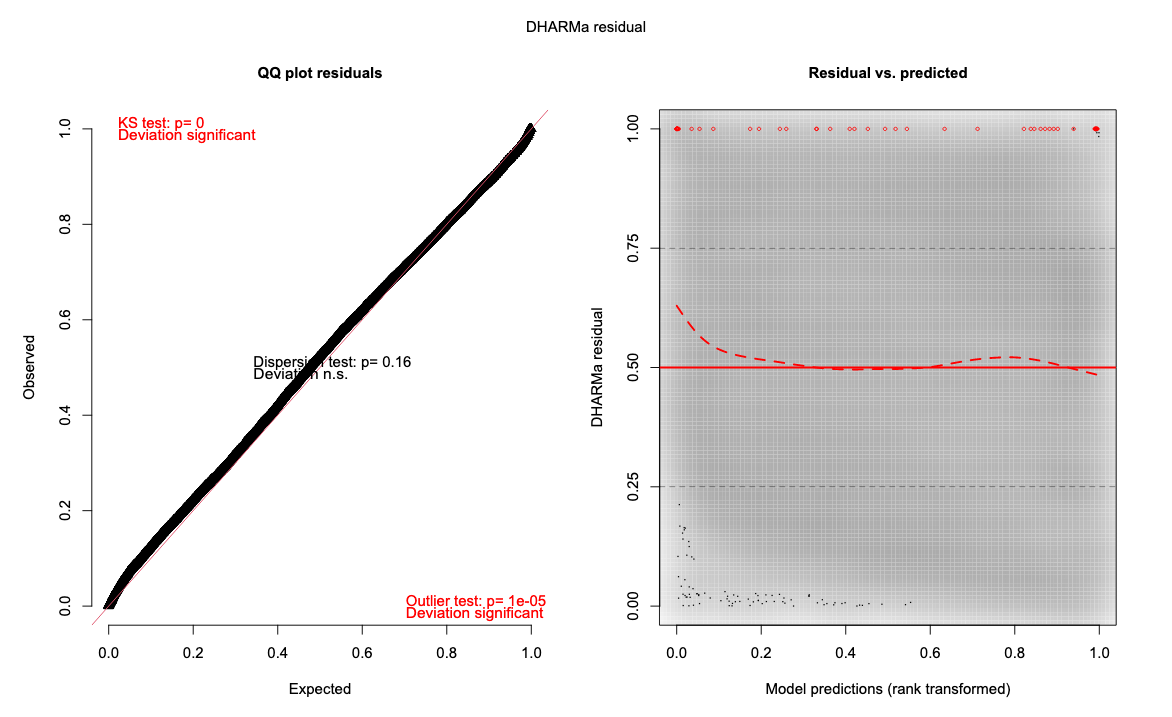
\includegraphics[width=\textwidth]{04_residual_analysis}
  \caption{Residual analysis for glmmTMB model.\label{fig:fig04_residual_analysis}}
\end{figure}


In order to understand how this ``feedback loop'' was developing, we fit
multiple regression models on our generated data. In the expression below,
\verb|pop| represents the popularity of a movie, \verb|t| represents the time
i.e. the iteration from 0 to 4, \verb|genre| represents the genre of a movie,
and \verb|movie_id| is the ID of a movie. Note that the genre was not used when
training the recommendation models described above, but it turned out that this
feature could explain a lot of the models' outputs.

\begin{verbatim}
  Family: nbinom2  ( log )
Formula:          pop ~ t * genre * rating + (1 | movie_id)
Data: features

     AIC      BIC   logLik deviance df.resid
 83863.8  84370.3 -41865.9  83731.8    15844

Random effects:

Conditional model:
 Groups   Name        Variance Std.Dev.
 movie_id (Intercept) 1.364    1.168
Number of obs: 15910, groups:  movie_id, 3182

Dispersion parameter for nbinom2 family ():   49

Conditional model:
                            Estimate Std. Error z value Pr(>|z|)
(Intercept)                -0.108714   0.272464  -0.399 0.689891
t                          -0.210272   0.021153  -9.941  < 2e-16 ***
genreAdventure              0.112129   0.574197   0.195 0.845174
genreAnimation             -2.286362   0.773873  -2.954 0.003132 **
genreChildren's             0.855196   0.755919   1.131 0.257915
genreComedy                -0.108159   0.352431  -0.307 0.758925
genreCrime                 -3.590470   0.850227  -4.223 2.41e-05 ***
genreDocumentary           -1.659325   1.508329  -1.100 0.271285
genreDrama                 -1.219969   0.409312  -2.981 0.002877 **
genreFilm-Noir            -16.633103   2.371128  -7.015 2.30e-12 ***
genreHorror                 0.512807   0.443025   1.158 0.247062
genreMusical               -4.259252   2.088483  -2.039 0.041410 *
genreMystery               -4.646920   1.461852  -3.179 0.001479 **
genreRomance               -2.118789   1.856289  -1.141 0.253699
genreSci-Fi                 0.363380   1.044431   0.348 0.727899
genreThriller               1.382908   0.855392   1.617 0.105944
genreWestern               -3.766758   2.108848  -1.786 0.074072 .
rating                      0.957533   0.085468  11.203  < 2e-16 ***
t:genreAdventure            0.161327   0.053403   3.021 0.002520 **
t:genreAnimation           -0.392012   0.067698  -5.791 7.01e-09 ***
t:genreChildren's           0.116028   0.066946   1.733 0.083068 .
t:genreComedy               0.119502   0.030504   3.918 8.94e-05 ***
t:genreCrime               -0.146821   0.085503  -1.717 0.085952 .
t:genreDocumentary          0.329357   0.195776   1.682 0.092507 .
t:genreDrama                0.005393   0.038739   0.139 0.889287
t:genreFilm-Noir           -0.730742   0.227275  -3.215 0.001303 **
t:genreHorror               0.148203   0.041813   3.544 0.000393 ***
t:genreMusical              0.265118   0.243060   1.091 0.275383
t:genreMystery             -1.150785   0.123034  -9.353  < 2e-16 ***
t:genreRomance              0.064921   0.227735   0.285 0.775590
t:genreSci-Fi              -0.311108   0.079779  -3.900 9.63e-05 ***
t:genreThriller             0.134758   0.077077   1.748 0.080403 .
t:genreWestern              0.184582   0.216581   0.852 0.394073
t:rating                    0.029594   0.006273   4.717 2.39e-06 ***
genreAdventure:rating      -0.209253   0.179840  -1.164 0.244606
genreAnimation:rating       0.594327   0.226301   2.626 0.008633 **
genreChildren's:rating     -0.473591   0.247951  -1.910 0.056131 .
genreComedy:rating         -0.194909   0.109223  -1.785 0.074341 .
genreCrime:rating           0.736375   0.243050   3.030 0.002448 **
genreDocumentary:rating    -0.113489   0.399299  -0.284 0.776242
genreDrama:rating          -0.031020   0.120957  -0.256 0.797601
genreFilm-Noir:rating       3.958891   0.595316   6.650 2.93e-11 ***
genreHorror:rating         -0.422452   0.151685  -2.785 0.005352 **
genreMusical:rating         0.944897   0.569196   1.660 0.096903 .
genreMystery:rating         1.092607   0.409047   2.671 0.007560 **
genreRomance:rating         0.013712   0.548422   0.025 0.980053
genreSci-Fi:rating         -0.423339   0.324094  -1.306 0.191477
genreThriller:rating       -0.729129   0.256016  -2.848 0.004400 **
genreWestern:rating         0.725673   0.578412   1.255 0.209625
t:genreAdventure:rating    -0.053250   0.015828  -3.364 0.000768 ***
t:genreAnimation:rating     0.110189   0.018603   5.923 3.16e-09 ***
t:genreChildren's:rating   -0.039499   0.020922  -1.888 0.059031 .
t:genreComedy:rating       -0.039790   0.008913  -4.464 8.04e-06 ***
t:genreCrime:rating         0.038460   0.022654   1.698 0.089557 .
t:genreDocumentary:rating  -0.088874   0.050610  -1.756 0.079076 .
t:genreDrama:rating        -0.006800   0.010754  -0.632 0.527202
t:genreFilm-Noir:rating     0.183567   0.054187   3.388 0.000705 ***
t:genreHorror:rating       -0.052874   0.013574  -3.895 9.81e-05 ***
t:genreMusical:rating      -0.082105   0.063538  -1.292 0.196285
t:genreMystery:rating       0.335177   0.032553  10.296  < 2e-16 ***
t:genreRomance:rating      -0.018634   0.064877  -0.287 0.773939
t:genreSci-Fi:rating        0.108210   0.023442   4.616 3.91e-06 ***
t:genreThriller:rating     -0.044310   0.022584  -1.962 0.049758 *
t:genreWestern:rating      -0.055461   0.056878  -0.975 0.329521
---
Signif. codes:  0 '***' 0.001 '**' 0.01 '*' 0.05 '.' 0.1 ' ' 1
\end{verbatim}

% Escrever o que eu fiz, sem preocupação com a formalidade. Mandar isso para o
% Patriota para ele lembrar do que a gente fez e marcar uma conversa para
% discutir se faz sentido e por onde a gente pode ir.
